%%%%%%%%%%%%%%%%%%%%%%%%%%%%%%%%%%%%
%% 
%% The End of the Middle Ages
%% 
%% Key Events:
%% 
%% 
%% Key Ideas:
%% 
%% 
%% Style: 
%% 
%% Figures:
%% A/M/L:
%% R/P/P:
%% 
%%%%%%%%%%%%%%%%%%%%%%%%%%%%%%%%%%%%

\firstslide[15 May 2012]{The End of the Middle Ages}

\section{14th Century Europe}
\begin{frame}{End of the Middle Ages}
	\includegraphics[height=2.6in]{map-13c-europe}
\end{frame}

\begin{frame}{How Many Popes?}
	\begin{itemize}
		\item<1->1309--1378. Papacy moved to Avignon.
		\item<2->1377. Pope Gregory XI moves back to Rome and promptly dies.
		\item<3->1378. Two popes elected by different sets of cardinals. Urban VI in Rome and Clement VII in France.
		\item<4->1378--1409. Multiple popes elected in both courts. Much confusion.
		\item<5->1409. Council of Pisa (the "Let's elect another pope!" council). Now, there are 3 popes. Confused yet?
		\item<6->1414--1417. Council of Constance. Cardinals decided they had more power than the Pope(s). 2 popes (the Italian ones) stepped down amicably. The Avignon Papacy continued its claim for a few more years.
	\end{itemize}
\end{frame}

\begin{frame}{Major Events}
	\begin{itemize}
		\item<1->1337--1453. Hundred Years' War between England and France.
		\item<2->c. 1348. Bubonic Plague across Europe.
		\item<3->1377. Jean Wycliff's translation of the Bible.
		\item<4->1390s. Chaucer's \emph{Canterbury Tales}.
		\item<4->1450s. Gutenberg's press and Bible.
	\end{itemize}
\end{frame}

\begin{frame}{Arts}
	\only<1>{
	\begin{center}
		Florence Cathedral (1298--1436)

		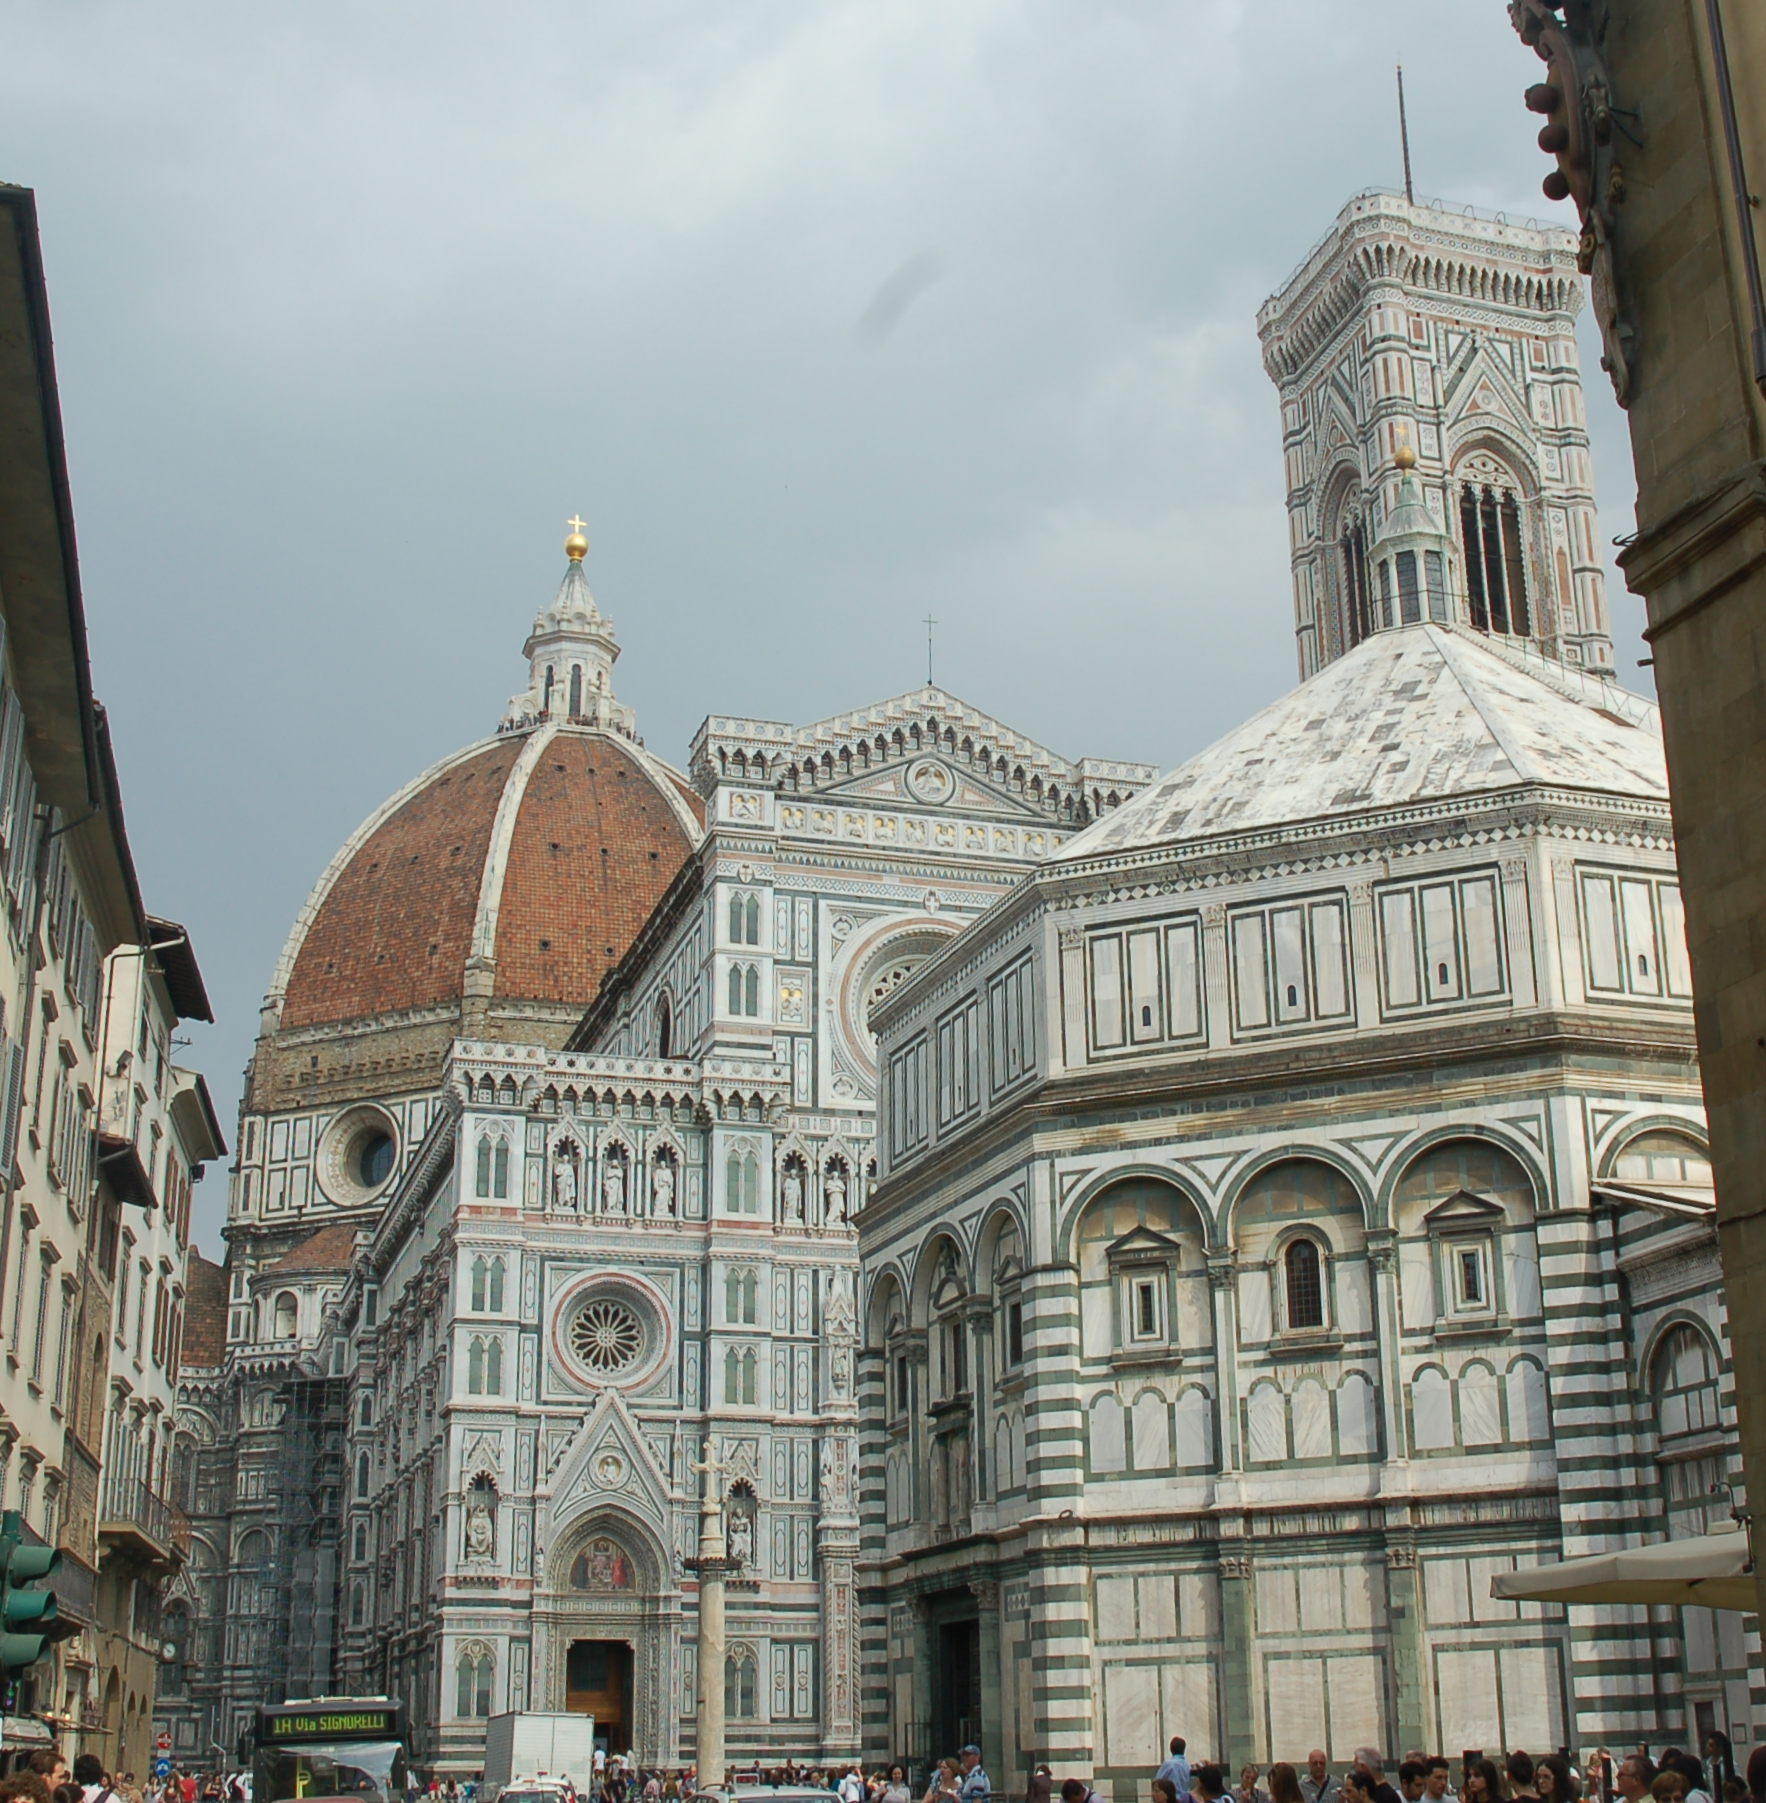
\includegraphics[height=2.6in]{img/img-florence.jpeg}
	\end{center}
	}
	\only<2>{
	\begin{center}
		Botticelli's Birth of Venus

		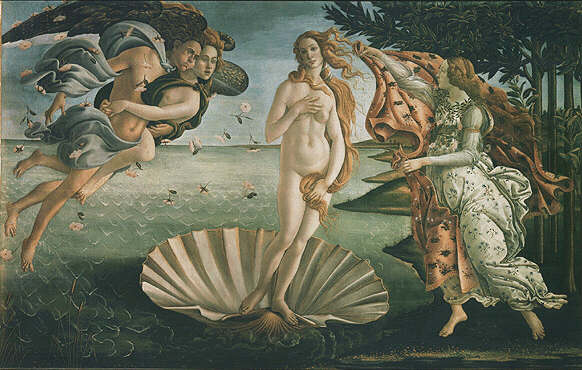
\includegraphics[height=2.3in]{img/img-venus.jpeg}
	\end{center}
	}
\end{frame}